
%http://mathematica.stackexchange.com/questions/11350/xkcd-style-graphs
\documentclass[12pt]{article}
%\usepackage{pseudocode}
%\usepackage{dirtree}
% \usepackage[utf8]{inputenc}
% \usepackage{listings,xcolor}

% \usepackage{soul}
% \usepackage{ulem}


\usepackage{tikz-cd}
\usepackage{amsmath}
\usepackage[most]{tcolorbox}


\DeclareMathOperator*{\argmin}{arg\,min}


\usepackage[linesnumbered,lined,boxed,commentsnumbered]{algorithm2e}
%\usepackage{algorithmicx}
\usepackage{algpseudocode}
\algrenewcommand\algorithmicwhile{\textbf{until}}
\SetKwInOut{Input}{input}
\SetKwInOut{Output}{output}



\usepackage[round,authoryear]{natbib}
%\usepackage[margin=1.0in]{geometry}
\usepackage{graphicx}
\usepackage{moreverb}
\usepackage{hyperref}
\newcommand\infNorm[1]{\left\lVert#1\right\rVert_\infty}
\newcommand\twoNorm[1]{\left\lVert#1\right\rVert_2}
\newcommand\someNorm[1]{\left\lVert#1\right\rVert}

\usepackage{mathtools}
\mathtoolsset{showonlyrefs}

\usepackage[english]{babel}
\usepackage[12hr,level]{datetime}
%\usepackage{datetime}
\usepackage{amsfonts}

\newcommand{\xgusst}[1]{x^{guess}_{#1}}
\newcommand{\xnxt}[1]{x^{next}_{#1}}
\newcommand{\znxt}[1]{z^{next}_{#1}}
\newcommand{\xlst}[1]{x^{last}_{#1}}
\newcommand{\zlst}[1]{z^{last}_{#1}}
\newcommand{\zgusst}[1]{z^{guess}_{#1}}
\newcommand{\xguss}{\xgusst{}}
\newcommand{\xtpguss}{x^{tp1guess}}


\newcommand{\iSet}{{\mathcal{I}_t}}

\newcommand{\posInt}{{\mathcal{N}^+}}
\newcommand{\Rn}[1]{{\mathcal{R}^{#1}}}
\newcommand{\numX}{{N_x}}
\newcommand{\numZ}{{N_z}}
\newcommand{\numEps}{{N_\epsilon}}
\newcommand{\numR}{{N_r}}
\newcommand{\numIters}{{K}}
\newcommand{\numTerms}{{N_{terms}}}
\newcommand{\numPts}{{N_{points}}}
\newcommand{\thePoints}{{\{(x_{t-1},\epsilon_t)^{1} \ldots (x_{t-1},\epsilon_t)^{\numPts}\}}}
\newcommand{\thePts}{{\mathcal{P}}}
%\newcommand{\ADRCE}{{\bf ADRCE}}
%\newcommand{\ADR}{{\bf ADR}}
\newcommand{\ADRCE}{\XZFunc}
\newcommand{\ADR}{\xzFunc}




\newcommand{\xtmEpsArg}{{x_{t-1},\epsilon_t}} 
\newcommand{\xtArg}{{x_{t} }}


\newcommand{\sumLinPart}{{
B x_{t-1}+ \phi \psi_\epsilon\epsilon + (I - F)^{-1} \phi \psi_c 
}}
\newcommand{\sumZPart}{{
 \sum_{\sForSum=0}^\infty F^s \phi z_{t+\sForSum}(x_{t-1},\epsilon) 
}}
\newcommand{\sumZPartZero}{{
 \phi z_{t}(x_{t-1},\epsilon) 
}}
\newcommand{\sumZPartPos}{{
 \sum_{\sForSum=1}^\infty F^s \phi Z_{t+\sForSum}(x_{t-1},\epsilon) 
}}

\newcommand{\EsumLinPart}{{
	 B x_{t-1}+ (I - F)^{-1} \phi \psi_c 
}}
\newcommand{\EsumZPartZero}{{
	  \sum_{\sForSum=0}^\infty F^s \phi Z^{PF}_{t+\sForSum}(x_{t-1},0) 
}}
\newcommand{\EsumZPartEpsilon}{{
	  \sum_{\sForSum=0}^\infty F^s \phi \expct{z_{t+\sForSum}(x_{t-1},\epsilon)}
}}
\newcommand{\EsumCapZPart}[1]{{
	  \sum_{\sForSum=0}^\infty F^s \phi {Z^{#1}_{t+\sForSum}(x_{t-1})}
}}
\newcommand{\uncnxpt}[2]{{\mathcal{E}\left [ \left . #1 \right | #2  \right ]}}
\newcommand{\expct}[1]{{\mathcal{E}\left [ #1 \right ]}}

\newcommand{\xzFuncGuess}{{\mathbb{g}}}
\newcommand{\xzFuncGuessIn}{{\mathbf{\mathbb{g}_{in}}}}
\newcommand{\genxzFuncGuessIn}{{\mathbf{gen\mathbb{g}_{in}}}}
\newcommand{\xzFuncGuessSig}{{(\Rn{\numX})\rightarrow
(\Rn{({\numX+\numZ})})}}


\newcommand{\xzFunc}{{{\gamma}}}
\newcommand{\xzFuncSig}{{(\Rn{\numX+\numEps})\rightarrow
(\Rn{({\numX+\numZ})})}}

\newcommand{\XZFunc}{{\mathbb{G}}}
\newcommand{\genXZFunc}{{\mathbf{gen\mathbb{G}}}}
\newcommand{\bigXFuncSig}{{(\Rn{\numX})\rightarrow
(\Rn{({\numX+\numZ})})}}


\newcommand{\genXGFP}{{\mathcal{U}}}
\newcommand{\xgFP}{{\mathcal{V}}}

\newcommand{\genFpf}{{\mathbf{gen}_\fpf}}
\newcommand{\fpf}{{\mathcal{T}}}
\newcommand{\fpfIn}{{\mathbf{t}_{in}}}
\newcommand{\fpfOut}{{\mathbf{t}_{out}}}
\newcommand{\genFpfIn}{{\mathbf{gen\fpf}_{in}}}
\newcommand{\genFpfOut}{{\mathbf{gen\fpf}_{out}}}

\newcommand{\genSlvr}{{\mathbf{gen}_{\slvr}}}
\newcommand{\slvr}{{\mathcal{S}}}
\newcommand{\slvrIn}{{\mathbf{s}_{in}}}
\newcommand{\slvrOut}{{\mathbf{s}_{out}}}
\newcommand{\genSlvrIn}{{\mathbf{gen\slvr}_{in}}}
\newcommand{\genSlvrOut}{{\mathbf{gen\slvr}_{out}}}
\newcommand{\solverSig}{{
\frfpnsRegimeFuncHelp
}}
\newcommand{\allArgs}{(x_{t-1},\epsilon,x_t,\expct{x_{t+1}})}
\newcommand{\proj}[1]{{\pi_{#1}}}
\newcommand{\eqnArg}{\mathbf{m}_{in}}
\newcommand{\eqnOut}{\mathbf{m}_{err}}
\newcommand{\eqnFunc}{\mathbb{M}}
\newcommand{\gate}{\mathbf{b}}
\newcommand{\eqnFuncSysIExpl}[1]{\{(\mathbf{b}_{#1}\allArgs,\eqnFunc_{#1}\allArgs=0) \}}
\newcommand{\eqnFuncSysI}[1]{\mathbb{C}_{#1}}
\newcommand{\eqnFuncSys}{\{\eqnFuncSysI{1},\ldots,\eqnFuncSysI{M}\}}
\newcommand{\eqnErrs}{{{m}_e}}
\newcommand{\eqnFuncSig}{{\Rn{3\numX+\numEps+\numZ}\rightarrow\Rn{\numX}}}


\newcommand{\lilXFuncSig}{{fix lilXFuncSig}}



\newcommand{\frfpnsFuncSig}{{\Rn{\numX+\numEps}\rightarrow\Rn{\numX+\numZ}}}

\newcommand{\bigXRegimeFuncSig}{{(\Rn{\numX+1})\rightarrow
(\Rn{({\numX+\numZ})})}}
\newcommand{\lilXRegimeFuncSig}{{(\Rn{\numX+1+\numEps+\numZ})\rightarrow
(\Rn{({3(\numX+1)+\numEps+\numZ})})}}
\newcommand{\eqnRegimeFuncSig}{{
\{\Rn{3(\numX+1)+\numEps+\numZ}\rightarrow\Rn{\numX},
\ldots,
\Rn{3(\numX+1)+\numEps+\numZ}\rightarrow\Rn{\numX}\}
}}
\newcommand{\frfpnsRegimeFuncHelp}{{\Rn{\numX+\numEps}\rightarrow\Rn{\numX+\numZ}}}

\newcommand{\frfpnsRegimeFuncSig}{{
\{ (\frfpnsRegimeFuncHelp{1}), \ldots ,  (\frfpnsRegimeFuncHelp{\numR})\}
}}

\newcommand{\dstSpec}{{\mathbf{distSpec}}}
\newcommand{\expctSpec}{{\mathbf{expctSpec}}}
\newcommand{\grdSpec}{{\mathbf{grdSpec}}}


\newcommand{\linMod}{{\mathcal{L}}}
\newcommand{\linModMats}{{\{H,\psi_\epsilon,\psi_c;B,\phi,F\}}}
\newcommand{\sForSum}{{\nu}}

\newcommand{\xWOarg}{   \mathbf{x}}
\newcommand{\xWarg}{   \mathbf{x}(x_{t-1},\epsilon)}
\newcommand{\xWargK}{   \hat{\mathbf{x}}(x_{t-1},\epsilon,k)}
\newcommand{\xWOargK}{   \hat{\mathbf{x}}}

\newcommand{\xpWOarg}{   \mathbf{x}^p}
\newcommand{\xpWarg}{   \mathbf{x}^p(x_{t-1},\epsilon)}
\newcommand{\xpWargK}{   \hat{\mathbf{x}}^p(x_{t-1},\epsilon,k)}
\newcommand{\xpWOargK}{   \hat{\mathbf{x}^p}}


\newcommand{\xppWOarg}{   \mathbf{x}^{p'}}
\newcommand{\xppWarg}{   \mathbf{x}^{p'}(x_{t-1},\epsilon)}
\newcommand{\xppWargK}{   \hat{\mathbf{x}}^{p'}(x_{t-1},\epsilon,k)}
\newcommand{\xppWOargK}{   \hat{\mathbf{x}^{p'}}}



\newcommand{\XWOarg}{   \mathbf{X}}
\newcommand{\XWarg}{   \mathbf{X}(x_{t-1},\epsilon)}
\newcommand{\XWargK}{   \hat{\mathbf{X}}(x_{t-1},\epsilon,k)}
\newcommand{\XWOargK}{   \hat{\mathbf{X}}}


\newcommand{\XpWOarg}{   \mathbf{X}^p}
\newcommand{\XpWarg}{   \mathbf{X}^p(x_{t-1},\epsilon)}
\newcommand{\XpWargK}{   \hat{\mathbf{X}^p}(x_{t-1},\epsilon,k)}
\newcommand{\XpWOargK}{   \hat{\mathbf{X}^p}}

\newcommand{\zWOarg}{   \mathbf{z}}
\newcommand{\zWarg}{   \mathbf{z}(x_{t-1},\epsilon)}
\newcommand{\zWargK}{   \hat{\mathbf{z}}(x_{t-1},\epsilon,k)}
\newcommand{\zWOargK}{   \hat{\mathbf{z}}}


\newcommand{\ZWOarg}{   \mathbf{Z}}
\newcommand{\ZWarg}{   \mathbf{Z}(x_{-1},\epsilon)}
\newcommand{\ZWargK}{   \hat{\mathbf{Z}}(x_{-1},\epsilon,k)}
\newcommand{\ZWOargK}{   \hat{\mathbf{Z}}}


\newcommand{\zpWOarg}{   \mathbf{z}^p}
\newcommand{\zpWarg}{   \mathbf{z}^p(x_{t-1},\epsilon)}
\newcommand{\zpWargK}{   \hat{\mathbf{z}^p}(x_{t-1},\epsilon,k)}
\newcommand{\zpWOargK}{   \hat{\mathbf{z}^p}}



\newcommand{\zppWOarg}{   \mathbf{z}^{p'}}
\newcommand{\zppWarg}{   \mathbf{z}^{p'}(x_{t-1},\epsilon)}
\newcommand{\zppWargK}{   \hat{\mathbf{z}^{p'}}(x_{t-1},\epsilon,k)}
\newcommand{\zppWOargK}{   \hat{\mathbf{z}^{p'}}}


\newcommand{\ZpWOarg}{   \mathbf{Z}^p}
\newcommand{\ZpWarg}{   \mathbf{Z}^p(x_{-1},\epsilon)}
\newcommand{\ZpWargK}{   \hat{\mathbf{Z}^p}(x_{-1},\epsilon,k)}
\newcommand{\ZpWOargK}{   \hat{\mathbf{Z}^p}}


\newcommand{\xIter}[2]{\mathcal{X}^{#1}(#2)}
\newcommand{\xNow}[1]{x^{#1}_t(x_{t-1},\epsilon_t)}
\newcommand{\zNow}[1]{z^{#1}(x_{t-1},\epsilon_t)}
\newcommand{\xNowtp}[1]{x^{#1}_{t+1}(x_{t-1},\epsilon_t)}
\newcommand{\XNow}[3]{\mathcal{X}^{#1}_{#2}(x_{#3})}
\newcommand{\ZNow}[3]{\mathcal{Z}^{#1}(x_{#3})}


\newcommand{\rcpC}{{\mathbf{N}}}


\newcommand{\gssaKtp}{{\left \{  
\beta \frac{u^\prime(c_{\tau+1})}{u^\prime(c_{\tau})} 
[1- \delta + a_{t+1}f^\prime(k_{\tau+1})]
\right \} -1}}


\newenvironment{myProof}[1][Proof]{\begin{trivlist}
  \item[\hskip \labelsep {\bfseries #1}]}{\end{trivlist}}
\newenvironment{myDefinition}[1][Definition]{\begin{trivlist}
\item[\hskip \labelsep {\bfseries #1}]}{\end{trivlist}}
\newenvironment{myExample}[1][Example]{\begin{trivlist}
\item[\hskip \labelsep {\bfseries #1}]}{\end{trivlist}}
\newenvironment{myRemark}[1][Remark]{\begin{trivlist}
\item[\hskip \labelsep {\bfseries #1}]}{\end{trivlist}}

\newcommand{\myQed}{\nobreak \ifvmode \relax \else
      \ifdim\lastskip<1.5em \hskip-\lastskip
      \hskip1.5em plus0em minus0.5em \fi \nobreak
      \vrule height0.75em width0.5em depth0.25em\fi}

\newcommand{\xtFuncTI}{\mathcal{X}(x,\epsilon)}
\newcommand{\XtFuncTI}{\mathbf{X}(x)}
\newcommand{\expctEps}[1]{\mathcal{E}_{\epsilon} \left [#1 \right ]}
\newcommand{\xsubtFunc}[2]{\mathcal{X}_{#1}{#2}}
\newcommand{\xtFunc}[1]{\mathcal{X}{#1}}
\newcommand{\XtFunc}[1]{\mathbf{X}{#1}}
\newcommand{\stochF}[1]{\mathcal{S}^{\{#1\}}}
\newcommand{\detF}[1]{\mathcal{D}^{\{#1\}}}
\newcommand{\initXE}{(x_{-1},\epsilon_0)}
\newcommand{\nlEqnLHS}[4]{
  h_\varpi(#1,#2,E_t(#3),\epsilon_#4)}

\newcommand{\nlEqn}[4]{
h_\varpi^{det}(#1,#2,\epsilon_#4)+
H_\varpi^{det}(#1,#2,\epsilon_#4)E_#4(#3)
}
\newcommand{\nlEqnSel}[4]{
\varpi=m_\varpi^{det}(#1,#2,\epsilon_#4)+
M_\varpi^{det}(#1,#2,\epsilon_#4)E_#4(#3)
}
\newcommand{\itSup}[1]{{\{#1\}}}
\newcommand{\initX}{(x)}
\newcommand{\initXEN}{(x_,\epsilon_t)}
\newcommand{\detComp}[1]{{\detF{K-\nu}( \cdots \detF{K-1}(\detF{K}(#1))))}}
\newcommand{\tArg}{(x_{t-1},\epsilon_t)}
\newcommand{\tNo}{(x_{t-1})}


\newtheorem{theorem}{Theorem}[section]


\newcommand{\fSum}{\mathcal{F}}
\newcommand{\modArgs}{\mathbb{X}}

\newcommand{\aSmolPoly}{p(x,\epsilon)}
\newcommand{\smolRngs}{\{(\underbar{x}_1,\bar{x}_1),\ldots,(\underbar{x}_L,\bar{x}_L),(\underbar{$\epsilon$}_1,\bar{\epsilon}_1),\ldots,(\underbar{$\epsilon$}_L,\bar{\epsilon}_K)\}}
\newcommand{\distribSpec}{\{f_1,\ldots,f_K\}}


%
\newcommand{\eulerE}{\mathbf{e}}

\title{A Series Representation for Dynamic Economic Model Solutions}

\date{\currenttime -- \today }


\newtheorem{theorem}{Theorem}[section]

\newenvironment{proof}[1][Proof]{\begin{trivlist}
  \item[\hskip \labelsep {\bfseries #1}]}{\end{trivlist}}
\newenvironment{definition}[1][Definition]{\begin{trivlist}
\item[\hskip \labelsep {\bfseries #1}]}{\end{trivlist}}
\newenvironment{example}[1][Example]{\begin{trivlist}
\item[\hskip \labelsep {\bfseries #1}]}{\end{trivlist}}
\newenvironment{remark}[1][Remark]{\begin{trivlist}
\item[\hskip \labelsep {\bfseries #1}]}{\end{trivlist}}

\newcommand{\qed}{\nobreak \ifvmode \relax \else
      \ifdim\lastskip<1.5em \hskip-\lastskip
      \hskip1.5em plus0em minus0.5em \fi \nobreak
      \vrule height0.75em width0.5em depth0.25em\fi}

\author{Gary S. Anderson\thanks{The analysis and conclusions set forth are those of the author and do not indicate concurrence by other members of the research staff or the Board of Governors. I would like to thank Luca Guerrieri, Christopher Gust, Hess Chung, Benjamin Johannsen  and Robert Tetlow for their comments and suggestions. }}




\begin{document}
\maketitle

\begin{abstract}


 
This paper proposes a new series representation for bounded
time invariant discrete time maps that can serve as a useful
component in solving dynamic economic models
It also  provides a formula
for computing accuracy bounds for any proposed time invariant model solution.

With the series representation for time invariant maps in hand,
the paper shows how to use the solution to a deterministic problem at
time t, to improve upon a proposed solutions for
any given dynamic economic models with occasionally
binding constraints or regime switching.   The error bounds from the
series representation help with determining algorithm convergence by
measures for determining the potential benefits
of further solution refinement


% In this context, it  facilitates exploiting the 
% ``law of iterated expectations'' in computing rational expectations solutions for models with occasionally binding constraints.


\end{abstract}

 \newpage
 \tableofcontents
 \newpage






\section{A Series Representation for A Bounded Family of Paths}
\label{sec:seri-repr-bound}

Consider a family of functions:
 \begin{gather}
   \xWarg \in{R^L}\,\text{ with }\,\infNorm{\xWarg}  \le \bar{\mathcal{X}}\,\,\forall t> 0 \label{fFamily}.
 \end{gather}
The $x_{-1}$ is an  $L$ dimensional state vector and $\epsilon$ is a $K$ dimensional ``shock'' vector that together index
individual trajectories for future state vectors.  
Each member of the family characterizes the evolution of a {\em deterministic} trajectory of values.\footnote{Subsequent sections describe how these deterministic trajectories are useful for representing a wide array stochastic model solutions.}





For any linear homogeneous 
$L$ dimensional 
deterministic 
system 
\begin{gather}
  	 H_{-1} x_{t-1} + H_0 x_t + H_1 x_{t+1}=0\label{hSystem}
\end{gather}
that produces  a unique stable solution, 
it is well known\ \citep{anderson10} that  inhomogeneous solutions 
\begin{gather}
	 H_{-1} x_{t-1} + H_0 x_t + H_1 x_{t+1}=\psi_\epsilon \epsilon +\psi_{c}
\intertext{ can be computed as}
x_t=B x_{t-1} + \phi \psi_\epsilon \epsilon + (I - F)^{-1} \phi \psi_c
\intertext{where}
\phi= (H_0 +H_1 B)^{-1}  \text{ and } \,\,F=-\phi H_1 
\end{gather}
It will be useful to collect the components of this representation for use in
subsequent sections of the paper.
Define $\linMod \equiv \linModMats$.


{\small
Now, given the trajectories \refeq{fFamily}, define 
$  z_{t}(x_{t-1},\epsilon)$ as  %\footnote{These $z$ functions will soon prove useful in an algorithm for computing unknown trajectories like \refeq{fFamily}.}:
{
  \begin{align}
  z_{t}(x_{t-1},\epsilon) \equiv& H_{-1} \mathcal{X}_{t-1}(x_{t-1},\epsilon) + \nonumber\\
& H_0 \mathcal{X}_{t}(x_{t-1},\epsilon) +  \label{defZ} \\
& H_1 \mathcal{X}_{t+1}(x_{t-1},\epsilon). \nonumber
  \end{align}
}

\begin{theorem}
	 \begin{gather}
	 \mathcal{X}_{t}(x_{t-1},\epsilon) =B x_{t-1}+ \phi \psi_\epsilon\epsilon + (I - F)^{-1} \phi \psi_c + \sum_{\sForSum=0}^\infty F^s \phi z_{t+\sForSum}(x_{t-1},\epsilon) \label{theSeries}
\intertext{and}
	 \mathcal{X}_{t+1}(x_{t-1},\epsilon) =B \mathcal{X}_{t} + \sum_{\sForSum =0}^\infty F^\sForSum \phi z_{t+\sForSum}(x_{t-1},\epsilon) + (I - F)^{-1} \phi \psi_c \,\,\,\forall t \ge  0.
	 \end{gather}
\end{theorem}
}
\begin{proof}
  For every bounded family of functions,
  $\mathcal{X}_t(x_{t-1},\epsilon_t)$, \citep{anderson10}  shows that for any given $x_{t-1},\epsilon_t$ this expression must be true.
Since the eigenvalues of F are all less than one and the $z$'s are bounded,
 the series always converges.
\end{proof}


	 Consequently, given a family of trajectories like those in \refeq{fFamily},
and a stable linear homogeneous system like \refeq{hSystem},
one can easily compute a series 
representation \refeq{theSeries} for any  bounded function generating a family of
trajectories.
Interestingly, the linear model, $H$, the  constant term $\psi_c$ and the
impact of the stochastic shocks $\psi_\epsilon $ can  be 
chosen rather arbitrarily -- the only costraint being the existence of a saddle-point solution or the linear system.  
The formula will provide a series  for any 
$L$ dimensional $\linMod$.
This observation will give us some confidence in the 
robustness of the algorithms described in section 
\ref{sec:unknown-solutions} for constructing series 
representations for unknown families of functions 
satisfying complicated systems of dynamic non-linear equations.



One could consider approximating $\mathcal{X}_t(x_{t-1},\epsilon)$ by 
truncating the series \ref{theSeries} at a finite number of terms.
 	 \begin{gather}
 	 \xWargK \equiv B x_{t-1}+ \phi \psi_\epsilon\epsilon + \sum_{s=0}^k F^s \phi z_{t}(x_{t-1},\epsilon) + (I - F)^{-1} \phi \psi_c \label{theTruncSeries}
 \end{gather}
We can bound the  series approximation truncation errors.
Since
    \begin{gather}
      \label{eq:1}
\sum_{s=k+1}^{\infty} F^s \phi \psi_z = (I -F)^{-1} F^{k+1}\phi \psi_z       \\
\infNorm{\xWarg-\xWargK} \le \infNorm{(I -F)^{-1} F^{k+1}\phi \psi_z} \left ( \infNorm{H_{-1} }+ \infNorm{H_{0} }+ \infNorm{H_{1} } \right )\bar{\mathcal{X}}
    \end{gather}
Note that for approximating $\xWarg$ the impact of  a given realization along the path declines for those realizations which are  more temporally distant.




\subsection{A Simple Example: An ``Almost'' Arbitrary Linear Model and an ``Almost'' Arbitrary Family of Solution Paths}
\label{sec:almostarbitrary}


Consider the following constructed from ``almost'' arbitrary coefficients
\begin{gather}
  \begin{bmatrix}
H_{-1}&H_{0}&H_{1} 
  \end{bmatrix}=
\vcenter{\hbox{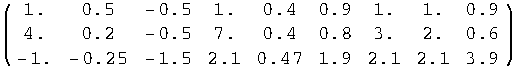
\includegraphics{refHmat.pdf}}}\intertext{with $\psi_c=\psi_\epsilon=0, \,\,  \psi_z=I$.
These coefficients are not completely arbitrary in so far as the series 
representation requires that the linear model
has a unique stable solution.}
  B=
\vcenter{\hbox{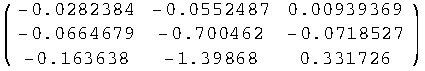
\includegraphics{refBmat.pdf}}}\\
\phi=
\vcenter{\hbox{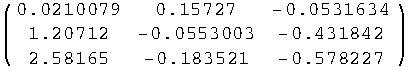
\includegraphics{refPhimat.pdf}}}\\
F=
\vcenter{\hbox{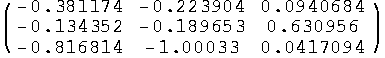
\includegraphics{refFmat.pdf}}}
\end{gather} 



The series representation requires that the state values along the 
paths remain bounded.  For example, consider the following three
bounded families of state vector paths.\footnote{See Section \ref{sec:arbitr-path-gener}
for a listing of the programs.}
The first set of trajectories is a multiple of
the digits in the decimal representation of $\pi$.  
determined by a nonlinear function of the initial conditions and the shock.
The second set of trajectories oscillates between two values
determined by  a nonlinear function of the initial conditions and the shock.
The third set of trajectories is a sequence of uniformly distributed random
numbers based on a seed determined by  a nonlinear function of  the initial conditions and the shock.
These examples paths were chosen to emphasize that the trajectories
 need not converge to a fixed point, and 
need not be produced by iteration of a discrete-time map.
The boundedness of the paths is a sufficient condition for the existence 
of the series representation.\footnote{Although useful in some contexts,
this paper will not investigate sufficient conditions for families of
unbounded trajectories.}



\begin{figure}
  \centering
\includegraphics[width=2in]{piPath.pdf}
\includegraphics[width=2in]{oscillPath.pdf}
\includegraphics[width=2in]{pseudoPath.pdf}

\includegraphics[width=3in]{theZs.pdf}
\includegraphics[width=3in]{arbTruncErr.pdf}  
\caption{RBC Truncation Error Bound Versus Actual}
  \caption{State Variables and the  z's Corresponding to  $x_{-1}=(1,2,3),\epsilon=(2,1,2)$} \label{arbFig}
\end{figure}


Figure \ref{arbFig} shows, for a particular initial state vector and shock value,  the paths for the state vectors and the corre z's that generate the path.
One can repeat the calculations for any given initial condition to produce
a z series exactly replicating the given set of trajectories.  The family
of z functions along with equation \ref{theSeries} provide a series 
representation for the family of trajectories.  Figure \ref{figArbTrunc} shows
that the truncation error bound is a very conservative measure of the accuracy
of the truncated series.  The series requires only the first 20 terms to compute
the initial value of the state vector to machine precision. 
The series representation can compute the entire series to machine precision
if all the terms are included, but the terms for state vectors closer 
to the initial time have the most important impact.


\begin{figure}
  \centering
  \caption{Error Bound Versus Actual Error} \label{figArbTrunc}
\end{figure}




\subsection{Example: A Simple RBC Model Example With Known Solution}
\label{sec:simple-rbc-model-2}


 {\bf RBC Model Example}
  See for example\cite{Maliar2005}
 \begin{gather*}
   \max\left \{  u(c_t^t) + E_t \sum_{\tau=t}^\infty \beta \delta^{\tau+1-t}u(c_{\tau+1}^t)\right \}\\
c_\tau^t + k_\tau^{t+1}=(1-d)k_\tau^{t-1} + \theta_\tau f(k_\tau^{t-1})\\
f(k_\tau^{t-1})= k_\tau^\alpha
 \end{gather*}

\begin{gather}
\frac{1}{c_t^{\eta}}=\alpha \delta k_{t}^{\alpha-1} E_t \left (\frac{\theta_{t}}{c_{t+1}^\eta} \right ) \\
c_t + k_t=\theta_{t-1}k_{t-1}^\alpha \\
 \theta_t =\theta_{t-1}^\rho e^{\epsilon_t}\label{rbcSys}
\intertext{for $\eta=1$}
\frac{1}{c_t}=\alpha \delta k_{t}^{\alpha-1} E_t \left (\frac{\theta_{t}}{c_{t+1}} \right ) \\
c_t + k_t=\theta_{t-1}k_{t-1}^\alpha \\
\theta_t =\theta_{t-1}^\rho e^{\epsilon_t}\label{rbcSys}
\intertext{and there is a closed form solution}
  k_{t}= \alpha \delta \theta_{t} k_{t-1}^\alpha.\label{soln}\\
c_t=  (1-\alpha \delta) \theta_{t} k_{t-1}^\alpha
\end{gather}
For mean zero iid $\epsilon_t$ we can easily compute a family of trajectories like \refeq{fFamily}
\begin{gather}
  \begin{bmatrix}
c_{t+s}(k_{t-1},\theta_t,\epsilon_t)\\k_{t+s}(k_{t-1},\theta_t,\epsilon_t)    \\ \theta_{t+s}(\theta_{t-1},\theta_t,\epsilon_t)    
  \end{bmatrix}
\intertext{with conditional mean converging over time to }
  \begin{bmatrix}
    c_{ss}\\k_{ss}
  \end{bmatrix}=
  \begin{bmatrix}
\nu^\alpha-\nu\\ \nu
  \end{bmatrix}\intertext{where}
\nu= \alpha ^{\frac{1}{1-\alpha }} \delta ^{\frac{1}{1-\alpha }}
\end{gather}


We can use the family of conditional expectations
along with the contrived reference model to recover an 
approximation for equation \refeq{soln} along with error bounds.
The series representation provides a weighted sum of z functions that give us
an approximation for the known solution.
\footnote{Note that the reference model is deterministic and the $z$ functions account for the stochastic nature of the model.}
% \footnote{
% We need not  make these adjustments for the steady state,
% but doing so economizes on the number of terms 
% required for a given level of approximation
% accuracy.}

Using the following parameter values

\begin{gather}
\vcenter{\hbox{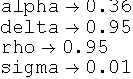
\includegraphics{RBCParamSubs.pdf}}} \,\, \text{ with } \,\,
  \begin{bmatrix}
    c_{ss}\\k_{ss} \\ \theta_{ss} \label{rbcparams}
  \end{bmatrix}=
\vcenter{\hbox{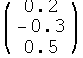
\includegraphics{RBCSSVal.pdf}}}
\end{gather}(\footnote{{RBCParamSubs.pdf}})(\footnote{{RBCSSVal.pdf}})


\begin{figure}
  \centering
\includegraphics{simpBoundsVActual.pdf}  
  \label{rbcTrunc}
  \caption{RBC Truncation Error Bound Versus Actual}
\end{figure}
\subsection{Constructing an Approximation: Problem Restatement}
\label{sec:constr-an-appr}



We will be interested in finding solutions for models that can be written in  the form


\begin{gather}
  h_i(x_{t-1},x_{t},x_{t+1},\epsilon_t)=h^{det}_{io}(x_{t-1},x_{t},\epsilon_t)+\sum_{j=1}^{p_i} [h^{det}_{ij}(x_{t-1},x_{t},\epsilon_t)h^{nondet}_{ij}(x_{t+1})]=0
\end{gather}
This is a very broad class of models and most economic models can 
be cast in this form.  

For example, the Euler equations for the  neoclassical growth  model 
\label{sec:simple-rbc-model-ext} can be written as
\begin{gather}
h_{10^{det}}(\cdot)=\frac{1}{c_t},\,\,
h_{11}^{det}()=\alpha \delta k_{t}^{\alpha-1} ,\,\,
h_{11}^{nondet}(\cdot)=E_t \left (\frac{\theta_{t+1}}{c_{t+1}} \right )\\
h_{20}^{det}(\cdot)=c_t + k_t-\theta_tk_{t-1}^\alpha,\,\,
h_{21}^{det}(\cdot)=0\\
h_{30}^{det}(\cdot)=\ln \theta_t -(\rho \ln \theta_{t-1} + \epsilon_t),\,\,
h_{31}^{det}(\cdot)=0
\end{gather}
Since we will be working with models where expectations are computed at time t, $\epsilon_t$ is known and the only stochastic components are those with time subscripts greater than $t$. We will need to compute 
the conditional expectation of nonlinear expressions,  
this specification will allow us to include auxiliary
variables that we will include in the augmented model for 
accurately recursively computing  the appropriate expected values.
Below, we will consider 
systems that augment these dynamic equations with additional constraints 
on the evolution of the variables.


We will be interested in
finding a time invariant function $g^\ast$ that satisfies
\begin{gather}
  \begin{split}
h(x_{t+s-1},g^\ast(x_{t+s-1},\epsilon_{t+s}),\mathcal{H}[g^\ast(g^\ast(x_{t+s-1},\epsilon_{t+s}),\epsilon_{t+s+1})],\epsilon_{t+s}) \label{theProblem} \\
%m(x_{t+s-1},g^\ast(x_{t+s-1},\epsilon_{t+s}),\mathcal{H}[g^\ast(g^\ast(x_{t+s-1},\epsilon_{t+s}),\epsilon_{t+s+1})],\epsilon_{t+s}) \ge 0  
  \end{split}
%  \intertext{define} 
% \mathcal{G}^\ast(x_{t+s-1},\epsilon_{t+s})= \mathcal{H}[g^\ast(g^\ast(x_{t+s-1},\epsilon_{t+s}),\epsilon_{t+s+1})] \nonumber
 \end{gather}
 for all $s>0$ where $\mathcal{H}$ is an operator, 
  that maps stochastic functions of $x$ and $\epsilon$ into deterministic 
functions of $x$ alone.  In this paper we will consider two such operators:



Could be any function that ``integrates out'' the $\epsilon$.
\footnote{What property, not the ``law of iterated expectations'' do I require.}
%so long as iterated ``expectations'' enforced.


\begin{description}
\item[Perfect Foresight]
\begin{gather}
     \mathcal{H}^{PF}[g^{k}(x,\epsilon_{t+T-k+1})]=
g^{k}(x,0)\\
\end{gather}


\item[Rational Expectations] 
\begin{gather}
     \mathcal{H}^{RE}[g^{k}(x,\epsilon_{t+T-k+1})]=
\mathcal{E}_t[g^{k}(x,\epsilon_{t+T-k+1})|x]\\
\end{gather}

 \end{description}












In what follows, we will use a representation like equation \refeq{theTruncSeries} 
to construct a sequence of functions, $g^k$, 
that will approximate the typically unknown solution $g^\ast$.
If we knew $g^\ast$, and  these function generate a bounded family of 
trajectories, we could define $z(x_{t+s-1},\epsilon_t)$ using \refeq{defZ}.
Constructing a companion linear model would subsequently allow 
 us to write down a series representation for the $g^\ast$ functions.  Below, we will show how to ``reverse engineer'' the series representation for $g^\ast$.






We begin by choosing some linear model of appropriate dimension that 
has a uniquely convergent steady state.  
Although this is not necessary, it may be possible to obtain this model by
linearizing the original model around the deterministic steady state.\footnote{As noted above, one could construct a series representation using any linear
 model of appropriate dimension with a unique stable solution.  The rate of convergence and the number of terms required for a  given level of accuracy will depend upon the linear model employed.}


 \begin{gather}
 g^0(x_{t-1},\epsilon_{t})=  
B x_{t-1}+ \phi \psi_\epsilon\epsilon_{t} +
 (I - F)^{-1} \phi \psi_c\\ \label{firstIter}
z^{0}_{t+i}(x_{t-1},\epsilon_{t-1})=0 \,\, \forall i \ge 0
 \end{gather}
We are now in a position to easily compute 
 \begin{gather}
\xIter{0}{x}=\mathcal{H}^{PF}[g^{0}(x,\epsilon_{t-k+1})]=
\mathcal{H}^{RE}[g^{0}(x,\epsilon_{t-k+1})]= 
B x+  (I - F)^{-1} \phi \psi_c
 \end{gather}
\begin{gather}
\underbrace{x_{t-1},0} 
\underbrace{\xNow{0},\zNow{0}}
\underbrace{\xNowtp{0}=\xIter{0}{x_{t}},0}
\end{gather}
In other words, from time t onwards, this approximation assumes 
that our stand-in
 convergent linear model completely characterizes the solution.\footnote{
The algorithm terminates with an approximation for 
the time invariant function $g^\ast$.}  It is unlikely that $g^0(x_{t-1},\epsilon_{t})$
satisfies equation \refeq{theProblem} for arbitrary $x_{t-1}$ even for $s=0$.
We can get a pessimistic upper bound for how far we are away from the solution 
by computing the infinity norm of substituting the variables from into Equation \refeq{theProblem}.
% \footnote{The values in Table \ref{truncTab} illustrate how
%pessimistic this approximation can be, but it turns out we can expect the accur%acy of  approximate truncation errors improve as we expand the approximation series.}

Next, we compute a solution in which the nonlinear equations are satisfied at time t alone while the stand-in linear system holds sway subsequently.
Our algorithm will  compute
\begin{gather}
\underbrace{x_{t-1},0} 
\underbrace{\xNow{1},\zNow{1}}
\underbrace{\xNowtp{1}=\xIter{1}{x_{t+1}},0}
\underbrace{\xNowtp{1}=\xIter{0}{x_{t+1}},0}
\end{gather}
that satisfy the nonlinear equation system at time t.
For a given $x_{t-1}$, we substitute
\begin{gather}
x_{t-1}, \,\,
  x_t=B x_{t-1} + \phi z^1(x_{t-1},\epsilon_t) , \,\,
  x_{t+1}=B x_{t} + \phi \mathcal{Z}^1(x_t)
\end{gather}
into the non linear equation system to determine the 
$z^1(x_{t-1},\epsilon_t)$ and consequently $x_t^1(x_{t-1},\epsilon_t)$.
We then have
 \begin{gather}
 g^1(x_{t-1},\epsilon_{t})=  
B x_{t-1}+ \phi \psi_\epsilon\epsilon_{t} +
\phi \psi_\epsilon z^1(x_{t-1},\epsilon_t)+
 (I - F)^{-1} \phi \psi_c\\ \label{firstIter}
z^{1}_{t+i}(x_{t-1},\epsilon_{t-1})=0 \,\, \forall i \ge 1
 \end{gather}
Now, $g^1(x_{t-1},\epsilon_{t})$
satisfies equation \refeq{theProblem} for arbitrary $x_{t-1}$ at time $t$ with $s=0$.  However, it probably does not solve the system for $s>0$.
We can get a pessimistic upper bound for how far we are away from the solution 
by substituting the variables and computing the infinity norm for plausible values of $x_{t-1}$.
\begin{gather}
\xNow{1},\xNowtp{1},\xNowtp{1}=\xIter{1}{x_{t+1}}
\end{gather}
into Equation \refeq{theProblem}. If the accuracy of the approximation is adequate, we need not compute any further  terms in the power series.  If not,
we are now in a position to compute our choice of
$\mathcal{Z}^1(x)=\mathcal{H}^{PF}[g^{1}(x,\epsilon_{t-k+1})]$ or
$\mathcal{Z}^1(x)=\mathcal{H}^{RE}[g^{1}(x,\epsilon_{t-k+1})]$.

%  \begin{gather}
%  g^0(x_{t-1},\epsilon_{t})=  
% B x_{t-1}+ \phi \psi_\epsilon\epsilon_{t} +
%  (I - F)^{-1} \phi \psi_c\\ \label{firstIter}
% z^{0}_{t+i}(x_{t-1},\epsilon_{t-1})=0 \,\, \forall i \ge 0
%  \end{gather}
%  \begin{gather}
%  g^0(x_{t-1},\epsilon_{t})=  
% B x_{t-1}+ \phi \psi_\epsilon\epsilon_{t} +
%  (I - F)^{-1} \phi \psi_c\\ \label{firstIter}
% z^{0}_{t+i}(x_{t-1},\epsilon_{t-1})=0 \,\, \forall i \ge 0
%  \end{gather}

Using these functions we can then compute a solution for a model whose trajectories satisfy equation system \refeq{rbcSys}
for two time periods and satisfy equation \refeq{rbcLinSys} subsequently.

\begin{gather}
\underbrace{x_{t-1},0}
\underbrace{\xNow{2},\zNow{2}} 
\underbrace{\xNowtp{2}=\XNow{2}{t}{t},\ZNow{2}{1}{t}}
\underbrace{\XNow{1}{t+1}{t},0}\underbrace{\XNow{0}{t+2}{t+1},0}    \intertext{where we have solved for $\xNow{2}$ and $\zNow{2}$ to satisfy the  equation system \refeq{theProblem}.}
\xNowtp{2}=\XNow{1}{t}{t}
\end{gather}

\begin{gather}
  \label{eq:1}
  x_t=B x_{t-1} + \phi z^2(x_{t-1},\epsilon) + F \phi \mathcal{Z}^1(x_t)\\
  x_{t+1}=B x_{t} + \phi \mathcal{Z}^1(x_t)+
 (I - F)^{-1} \phi \psi_c\\
  x_{t+2}=B x_{t+1} + (I - F)^{-1} \phi \psi_c\\
  x_{t+3}=B x_{t+2} + (I - F)^{-1} \phi \psi_c
\end{gather}

The next iteration highlights an aspect of the algorithmic step which allows us
to continue to exploit something not the ``law of iterated expectations''
%the law of iterated expectations in discovering the solution for the model.
{\small
\begin{gather}
\underbrace{x_{t-1},0}
\underbrace{\xNow{3},\zNow{3}} 
\underbrace{\xNowtp{3}=\XNow{3}{t}{t},\ZNow{3}{1}{t}} 
\underbrace{\XNow{2}{t+1}{t},\ZNow{2}{2}{t+1}} 
\underbrace{\XNow{1}{t+3}{t+2},0}
\underbrace{\XNow{0}{t+4}{t+3},0}
\end{gather}
}

\begin{gather}
  \label{eq:1}
  x_t=B x_{t-1} + \phi z^3(x_{t-1},\epsilon) + F \phi \mathcal{Z}^2(x_t)+ F^2 \phi \mathcal{Z}^1(x_t)+
 (I - F)^{-1} \phi \psi_c\\
  x_{t+1}=B x_{t} + \phi \mathcal{Z}^1(x_t)+ F^2 \phi \mathcal{Z}^1(x_t)+
 (I - F)^{-1} \phi \psi_c\\
  x_{t+2}=B x_{t+1} + (I - F)^{-1} \phi \psi_c\\
  x_{t+3}=B x_{t+2} + (I - F)^{-1} \phi \psi_c\\
  x_{t+4}=B x_{t+2} + (I - F)^{-1} \phi \psi_c
\end{gather}



In the general iteration step we will have
\begin{gather}
  \label{eq:1}
  x_t=B x_{t-1}  \phi \psi_\epsilon \epsilon_t + (I - F)^{-1} \phi \psi_c +
\sum_{s=0}^{k} F^s \phi \mathcal{Z}^{k-s}(x_{t+s}^{k+1})\\
  x_{t+s}^{k+1}=\Pi_{s=0}^k \xIter{s}{ x_{t}^{k+1}}
\end{gather}



Needs generalization of ``chunk'' $\frac{1}{c_t}\rightarrow \left (\frac{\theta_{t+1}}{c_{t+1}^\eta} \right )$

We construct our stand-in model by augmenting the model with the equation
\begin{gather}
  \rcpC_t=\frac{1}{c_t}
\end{gather}
substituting $\rcpC_{t+1}$ for $\frac{1}{c_{t+1}}$ in the first equation and 
 linearizing the RBC model about the ergodic mean
given in \refeq{rbcparams}
\begin{gather}
  \begin{bmatrix}
H_{-1}&H_{0}&H_{1} 
  \end{bmatrix}=
\vcenter{\hbox{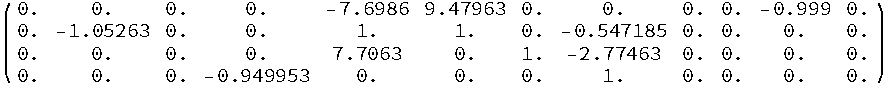
\includegraphics{RBCHmatSymb.pdf}}} \label{rbcLinSys}
\intertext{with}
\psi_\epsilon=
\begin{bmatrix}
  0\\0\\1\\0
\end{bmatrix}, \psi_z=I
\end{gather}(\footnote{generated by AMAPaperCalcs.mth {RBCHmatSymb.pdf}})

These coefficients  produce a unique stable linear solution.

\begin{gather}
  B=
\vcenter{\hbox{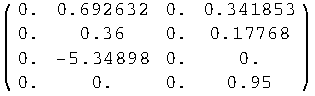
\includegraphics{RBCBmatSymb.pdf}}},
\phi=
\vcenter{\hbox{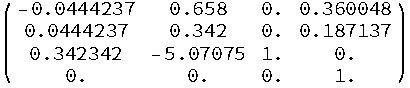
\includegraphics{RBCPhimatSymb.pdf}}}\\
F=
\vcenter{\hbox{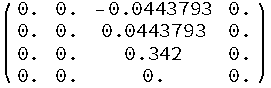
\includegraphics{RBCFmatSymb.pdf}}}\\
\psi_c=
\vcenter{\hbox{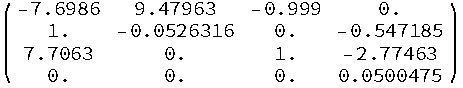
\includegraphics{RBCHSum.pdf}}}
\vcenter{\hbox{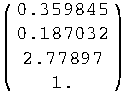
\includegraphics{RBCSS.pdf}}}=\vcenter{\hbox{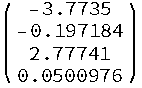
\includegraphics{RBCPsissSymb.pdf}}}
\end{gather}(\footnote{generated by AMAPaperCalcs.mth {RBCBmatSymb.pdf}})(\footnote{generated by AMAPaperCalcs.mth {RBCPhimatSymb.pdf}})(\footnote{generated by AMAPaperCalcs.mth {RBCFmatSymb.pdf}})(\footnote{generated by AMAPaperCalcs.mth {RBCHSum.pdf}})(\footnote{generated by AMAPaperCalcs.mth {RBCSS.pdf}})

Applying the formula \refeq{firstIter} produces:

{\tiny
\begin{gather}
  \begin{bmatrix}
c_t\\k_t\\ \rcpC_t\\\theta_t
  \end{bmatrix}=%paperCalcsRBCExample xt00
   \left(
   \begin{array}{c}
 0.359845 \epsilon _t+0.692632 k_{t-1}+0.341853 \theta _{t-1}-0.0442851
   \text{z1}_{t-1}+0.658 \text{z2}_{t-1}+0.359845 \text{z3}_{t-1}-0.111552 \\
 0.187032 \epsilon _t+0.36 k_{t-1}+0.17768 \theta _{t-1}+0.0442851
   \text{z1}_{t-1}+0.342 \text{z2}_{t-1}+0.187032 \text{z3}_{t-1}-0.0579799 \\
 -5.34898 k_{t-1}+0.342 \text{z1}_{t-1}-5.08153
   \text{z2}_{t-1}+\text{z4}_{t-1}+3.7794 \\
 \epsilon _t+0.95 \theta _{t-1}+\text{z3}_{t-1}+0.05 \\
   \end{array}
   \right)
\end{gather}
}

and 


{\tiny
%xt01=Private`computeNextXt[{Private`bmat,Private`phimat,Private`fmat,Private`psieps,Private`psic,Private`psiz},solnFunc00PF[[3+Range[3]]],{{cc},{kk},{tt}},{1}]//N//Expand//Simplify
\begin{gather}
  \begin{bmatrix}
c_{t+1}\\k_{t+1}\\ \rcpC_{t+1}\\\theta_{t+1}
  \end{bmatrix}=%paperCalcsRBCExample xt00
  \left(
   \begin{array}{c}
 0.471397 \epsilon _t+0.249347 k_{t-1}+0.447827 \theta _{t-1}+0.0306732
   \text{z1}_{t-1}+0.23688 \text{z2}_{t-1}+0.471397 \text{z3}_{t-1}-0.134618 \\
 0.245012 \epsilon_t+0.1296 k_{t-1}+0.232761 \theta _{t-1}+0.0159426
   \text{z1}_{t-1}+0.12312 \text{z2}_{t-1}+0.245012 \text{z3}_{t-1}-0.0699687 \\
 -1.00043 \epsilon _t-1.92563 k_{t-1}-0.950409 \theta _{t-1}-0.23688
   \text{z1}_{t-1}-1.82935 \text{z2}_{t-1}-1.00043 \text{z3}_{t-1}+4.08954 \\
 0.95 \epsilon _t+0.9025 \theta _{t-1}+0.95 \text{z3}_{t-1}+0.0975 \\
   \end{array}
   \right)
\end{gather}}

Substituting  these expressions into equation \refeq{rbcSys} produces
a deterministic system such that, given specific values for 
$(x_{t-1},\epsilon_{t})=(c_{t-1}, k_{t-1},\rcpC_{t-1}, \theta_{t-1}, \epsilon_t)$, we can solve for $z_{1t}(x_{t-1},\epsilon_{t})$, $z_{2t}(x_{t-1},\epsilon_{t})$, $z_{2t}(x_{t-1},\epsilon_{t})$, and $z_{4t}(x_{t-1},\epsilon_{t})$  completely determining
$c_{t}(x_{t-1},\epsilon_{t})$, $k_{t}(x_{t-1},\epsilon_{t})$, $\rcpC_{t}(x_{t-1},\epsilon_{t})$  and $\theta_{t}(x_{t-1},\epsilon_{t})$.\footnote{In this example, the lagged value,  $c_{t-1}$ does not appear in the equation system and consequently plays no role in determining the solution.}  In effect we have 
computed a solution for a model whose trajectories satisfy equation system \refeq{rbcSys}
for one time period and satisfy equation \refeq{rbcLinSys} subsequently. As can
be seen in the top panel of Figure \ref{fig:cfuncfirst}, 
imposing the constraint for even a single period captures much of the non linearity, but the bottom panel shows that the solution is 
still significantly far away from the exact solution.


Number of function evaluations and time.

fixed point not necessary.

find root must use genxz func
takes time to construct function for findroot  called twice by fixed point, but solution guaranteed on second call.

%\includegraphics[height=8.0in]{conExpPathsNote.pdf}(\footnote{{conExpPathsNote.pdf}})



Took 0.01 seconds while profiling.  Findroot called the xz func about 30 times.
\begin{figure}
  \centering
%\includegraphics{cFuncExt00Lin.pdf}(\footnote{{cFunc00Lin.pdf}})
  \caption{Solution for c imposing non linear model constraints for a single period}
%\includegraphics{cFuncExt00Exact.pdf}(\footnote{{cFunc00Exact.pdf}})
  \caption{Solution for c imposing non linear model constraints for a single period}
  \label{fig:cfuncfirst}
\end{figure}

We are now in a position to compute
$\mathcal{H}^{PF}[g^{0}(x,\epsilon_{t-k+1})]$ or
$\mathcal{H}^{RE}[g^{0}(x,\epsilon_{t-k+1})]$.
Using these functions we can then compute a solution for a model whose trajectories satisfy equation system \refeq{rbcSys}
for two time periods and satisfy equation \refeq{rbcLinSys} subsequently.
\begin{gather}
  \label{eq:1}
  x_t=B x_{t-1} + \phi z_0(x_{t-1},\epsilon) + F \phi \mathcal{Z}^1(x_t)\\
  x_{t+1}=B x_{t} + \phi \mathcal{Z}^1(x_t)
\end{gather}
{\tiny

\begin{gather}%paperCalcsRBCExample.mth xt01
  \label{eq:2}
   \left(
   \begin{array}{c}
 0.359845 \epsilon _t+0.692632 k_{t-1}+0.341853 \theta _{t-1}-0.0442851
   \text{z1}_{t-1}-0.0442851 \text{Z1}_{t-1}+0.658 \text{z2}_{t-1}+0.359845
   \text{z3}_{t-1}+0.225036 \text{Z3}_{t-1}-0.0151455 \text{Z4}_{t-1}-0.111552 \\
 0.187032 \epsilon _t+0.36 k_{t-1}+0.17768 \theta _{t-1}+0.0442851
   \text{z1}_{t-1}+0.0442851 \text{Z1}_{t-1}+0.342 \text{z2}_{t-1}+0.187032
   \text{z3}_{t-1}-0.225036 \text{Z3}_{t-1}+0.0151455 \text{Z4}_{t-1}-0.0579799 \\
 -5.34898 k_{t-1}+0.342 \text{z1}_{t-1}+0.342 \text{Z1}_{t-1}-5.08153
   \text{z2}_{t-1}-1.73788 \text{Z3}_{t-1}+\text{z4}_{t-1}+0.116964
   \text{Z4}_{t-1}+3.7794 \\
 \epsilon _t+0.95 \theta _{t-1}+\text{z3}_{t-1}+0.05 \\
   \end{array}
   \right)
\end{gather}
}

{\tiny
  \begin{gather}
    \label{eq:3}
       \left(
   \begin{array}{c}
 0.471397 \epsilon _t+0.249347 k_{t-1}+0.447827 \theta _{t-1}+0.0306732
   \text{z1}_{t-1}-0.0578969 \text{Z1}_{t-1}+0.23688 \text{z2}_{t-1}+0.658
   \text{Z2}_{t-1}+0.471397 \text{z3}_{t-1}+0.429014 \text{Z3}_{t-1}-0.00465525
   \text{Z4}_{t-1}-0.134618 \\
 0.245012 \epsilon _t+0.1296 k_{t-1}+0.232761 \theta _{t-1}+0.0159426
   \text{z1}_{t-1}+0.104513 \text{Z1}_{t-1}+0.12312 \text{z2}_{t-1}+0.342
   \text{Z2}_{t-1}+0.245012 \text{z3}_{t-1}-0.119017 \text{Z3}_{t-1}+0.0205979
   \text{Z4}_{t-1}-0.0699687 \\
 -1.00043 \epsilon _t-1.92563 k_{t-1}-0.950409 \theta _{t-1}-0.23688
   \text{z1}_{t-1}+0.44712 \text{Z1}_{t-1}-1.82935 \text{z2}_{t-1}-5.08153
   \text{Z2}_{t-1}-1.00043 \text{z3}_{t-1}-0.534171 \text{Z3}_{t-1}+1.03595
   \text{Z4}_{t-1}+4.08954 \\
 0.95 \epsilon _t+0.9025 \theta _{t-1}+0.95 \text{z3}_{t-1}+\text{Z3}_{t-1}+0.0975 \\
   \end{array}
   \right)
  \end{gather}
}





\begin{figure}
  \centering
%\includegraphics{cFuncTwoPerErr.pdf}(\footnote{{cFuncTwoPerErr.pdf}})
 \caption{Solution for c imposing non linear model constraints for two periods}
%\includegraphics{cFuncThreePerErr.pdf}(\footnote{{cFuncThreePerErr.pdf}})
  \caption{Solution for c imposing non linear model constraints for three periods}
  \label{fig:cfuncsecond}
\end{figure}

\subsubsection{Approximating the Known Solution: $U(c) = Log(c)$ }
\label{sec:recov-known-solut}

\subsubsection{Approximating an Unknown Solution: $U(c) \ne Log(c)$ }
\label{sec:unknown-solutions}

\subsubsection{Occasionally Binding Constraints}
\label{sec:obc-solut}


\subsubsection{A Regime Switching Version}
\label{sec:regime-switch-model}



\cite{foerster13}

\begin{gather}
c_t + z_t k_t = z_t^{1-\alpha} k_{t-1}^\alpha + (1-\delta)k_{t-1}\\
 \log z_t = (1-\rho(s_t))\mu(s_t) + \rho(s_t)\log z_{t-1}+ \sigma(s_t) \epsilon_t\\
 c_t^{\gamma-1} = \beta  
 E_t ( c_{t+1}^{\gamma-1} (\alpha z_{t+1}^{1-\alpha} k_t^{\alpha -1} + (1-\delta) ))
\end{gather}

Compressing objects: 100% (7/7), done.
Writing objects: 100% (7/7), 11.85 KiB, done.


\begin{itemize}
\item do compositions in place instead of stacking
\item Use derivatives in approximation to solve illustrates how expectations ``smooth'' out the function ``kinks''
\item time invariance and constraints on paths
\item perturbation techniques on $x+{t-1}, \epsilon$
\item $\epsilon$ could be any exogenous even time varying factor
\item compute derivative of composition of function and use in update of decision rule from path errors
\item add diagnostic tests to checkLinMod checkMod
\item specify model definition requirements 
\item exploit linearity get derivative for update
\item generate a ``differential equation''
\item makeDRFunc and reconcile assessment and update code
\item use composition instead of stacking make interpolation decision rule pair
\item way to use centered and backward sums of z's
\item use derivative of sum and integral in update of function
\item time invariance iteration constraints on z's and paths
\item time invariance and function updates
\item $z(x,\epsilon,y)$? just need y ``exogenous''  y discrete, continuous, stochastic
\item progress monitor
\item big shocks abort linear liftoff good cautionary example
\item parallel
\item smolyak
\item constraint
\item regime
\item error messages
\item lucamod big shock
\item how to ``snug up'' solution using global feature of AMA series
\item linearity of representation and updating
\item deprecate path extension
\item fact that are decision rule constrains z's How? z's are all part of a decision rule uniqueness topology
\item one step defines all values  --  this should be exploitable
\item decision rule differs slightly from conditional expetation that gets iterated shock puts you on a path
\item mention possible to use Sims inputs
\item continuous time
\item $\Delta(x_{t-1},\epsilon_t) \implies \Delta Z(x_{t-1}) \implies PATH \implies NewZs$
\item suspect there is a corresponding PDE that may be easy to solve numerically
\item problem probably already solved in topology ( category theory )
\item perhaps can approx the exact PDE by using just a few terms
\item for time invariant map just need to get one step right so shouldn't need to worry about iterated compositions in formula for differential equaiton
\item Euler residuals like Luca and other measures like Villaverde use maliar measures 
\item findroot, nsolve other for deterministic problem
\item use all equations ==
\item nsolve choose multiple --  more constraints
\item \href{mathematica nsolve info}{http://mathematica.stackexchange.com/questions/47112/what-algorithms-does-nsolve-use}
\item \href{some choices}{http://mathematica.stackexchange.com/questions/40543/methods-for-nsolve}
  \begin{itemize}
  \item "EndomorphismMatrix"
"CompanionMatrix"
\item 
"Legacy"
\item 
"Aberth"
\item 
"JenkinsTraub"
  \end{itemize}
\item do maliar exercises
\item do rubio exercises
\item do luca exercises
\item equations CompiledFunction if findroot
\item equations Function if NSolve
\item java minimizer with constraints 
\item $dr1 = \sum ... z_1, dr2 = \sum ... z_2,,, dr2 - dr1= \sum ... (z_2-z_1)$
\item $dr_\ast - dr1= \sum ... (z_\ast-z_1)$
\item warnings about extrapolation
\item generate PDE
\item time invariance constraints on zs 
\item $ \Delta z \implies \Delta z \implies \Delta path$
\item implement derivative
\item functions with through can likely be parallelized also maps
\item kernel fireup time?
\item behavior when multiple solutions and when no solutions
\item how best to associate eqnFuncs with lilxkzkfunc 
\item multistep iterateions should match steady state solution exactly (see 
AMASeriesRepresentationExamples notebook for developing derivatives
\item should develop a test suite demonstrating identities satisfied
\item update path using newton step,  Stack` $\frac{\partial Z()}{\partial x_{t-1}}$
\item verify chunks can have t-1 and t  values
\item solve closed form example in one verifying iteration
\item ``pruned'' perturbation solution for initial guess at cond exp
\item can use to assess ``pruned'' perturbation solution
\item just collocation could be projection
\item make sure multiple shocks okay; implementation versus theoretical constraint
\item  could use different linmods for each regime
\item inits for nsolve, handholding for nsolve
\item improve monitors for misapplied functions
\item nsolve about 500 times a long as findroot
\item any time invariant dr with bounded solutions can be written as a series proof by construction
\end{itemize}
`	
\newpage
\appendix

\section{Arbitrary Path Generator Programs}
\label{sec:arbitr-path-gener}

\listinginput{1}{arbGenPath.mth}

\section{Program Signatures}
\label{sec:program-listings}
\begin{tabular}{|l|c|}
\hline
Number of $x_t$ variables&$\numX$\\
\hline
Number of $z_t$ variables&$\numZ$\\
\hline
Number of $\epsilon_t$ variables&$\numEps$\\
\hline
Number of regimes variables&$\numR$\\
\hline
Number of recursive iterations&$\numIters$\\
\hline
Interpolation Grid Specification&$\dstSpec$\\
\hline
Shock Distributions  Specification&$\dstSpec$\\
\hline
The Linear Reference Model&$\linMod\equiv\linModMats$\\  
\hline
Model Equation Function&$\eqnFuncSig$\\
\hline
\end{tabular}
\subsection{genLilXkZkFunc}
\label{sec:genlilxkzkfunc}
\begin{gather*}
\linMod \times \{  \bigXFuncSig, k \} \times \Rn{(\numX+\numEps)} \rightarrow
huh%\lilXFuncSig
\end{gather*}

\subsection{genFRFunc,genNSFunc}
\label{sec:genfrfunc}


\begin{gather*}
\{\numX,\numEps,\numZ\}\times(\lilXFuncSig)\times (\eqnFuncSig)    \rightarrow\\
\frfpnsFuncSig
\end{gather*}



\subsection{genFPFunc}
\label{sec:genfpfunc}
\begin{gather*}
\linMod \times \{  \bigXFuncSig, k \} \times (\eqnFuncSig)    \rightarrow\\ 
\frfpnsFuncSig
\end{gather*}




\subsection{genXZREInterpFunc}
\label{sec:genfpfunc}
\begin{gather*}
\{\numX,\numEps,\numZ\}\times(\lilXFuncSig)\times \grdSpec \times  \dstSpec   \rightarrow\\
\bigXFuncSig
\end{gather*}



\subsection{doIterREInterp}
\label{sec:doiterreinterp}

\begin{gather*}
  \linMod \times 
w\{(\lilXFuncSig)_1,\ldots,(\lilXFuncSig)_{\numR}\}  \\
 \times (\eqnFuncSig ) \times \grdSpec \times \dstSpec \rightarrow\\
\{\frfpnsFuncSig, \{(\lilXFuncSig)_1,\ldots,(\lilXFuncSig)_{\numR}\}\}
\end{gather*}



\subsection{nestIterREInterp}
\label{sec:nestiterreinterp}



\begin{gather*}
  \linMod \times 
\{(\lilXFuncSig)_1,\ldots,(\lilXFuncSig)_{\numR}\}  \\
 \times (\eqnFuncSig ) \times \grdSpec \times \dstSpec \times \numIters \rightarrow\\
\{\frfpnsFuncSig, \{(\lilXFuncSig)_1,\ldots,(\lilXFuncSig)_{\numR}\}\}
\end{gather*}



\subsection{genLilXkZkRegimeFuncs}
\label{sec:genlilxkzkregimefunc}
{\small
\begin{gather*}
\linMod \times \{(\{  \bigXFuncSig, k_i \})_{k_i=1},\ldots,(\{  \bigXFuncSig, k_i \})_{k_i=\numR}\} \times\\ \Rn{(\numX+\numEps)} \rightarrow\\
\{(\lilXRegimeFuncSig)_1,\ldots,(\lilXFuncSig)_{\numR}\}
\end{gather*}
}





\subsection{genFRRegimeFuncs, genNSRegimeFuncs}
\label{sec:genfrregimefunc}



{\small
\begin{gather*}
\{\numX,\numEps,\numZ\}\times\\
\{(\lilXRegimeFuncSig)_1,\ldots,(\lilXFuncSig)_{\numR}\}  \\
 \times (\eqnRegimeFuncSig )\rightarrow\\
\frfpnsRegimeFuncSig
\end{gather*}
}








\subsection{genFPRegimeFuncs}
\label{sec:genfpregimefunc}




{\small
\begin{gather*}
\{\numX,\numEps,\numZ\}\times\\
\{(\lilXRegimeFuncSig)_1,\ldots,(\lilXFuncSig)_{\numR}\}  \\
 \times (\eqnRegimeFuncSig )\rightarrow\\
\frfpnsRegimeFuncSig
\end{gather*}
}




\subsection{genXZREInterpRegimeFuncs}
\label{sec:genfpfunc}
\begin{gather*}
\{\numX,\numEps,\numZ\}\times(\lilXFuncSig)\times \dstSpec \times  \expctSpec   \rightarrow\\
\frfpnsFuncSig
\end{gather*}



\subsection{doIterREInterpRegime}
\label{sec:doiterreinterp}

\begin{gather*}
  \linMod \times 
w\{(\lilXRegimeFuncSig)_1,\ldots,(\lilXFuncSig)_{\numR}\}  \\
 \times (\eqnRegimeFuncSig ) \times \grdSpec \times \dstSpec \rightarrow\\
\{\frfpnsRegimeFuncSig, \{(\lilXRegimeFuncSig)_1,\ldots,(\lilXFuncSig)_{\numR}\}\}
\end{gather*}



\subsection{nestIterREInterpRegime}
\label{sec:nestiterreinterp}



\begin{gather*}
  \linMod \times 
w\{(\lilXRegimeFuncSig)_1,\ldots,(\lilXFuncSig)_{\numR}\}  \\
 \times (\eqnRegimeFuncSig ) \times \grdSpec \times \dstSpec  \times \numIters \rightarrow\\
\{\frfpnsRegimeFuncSig, \{(\lilXRegimeFuncSig)_1,\ldots,(\lilXFuncSig)_{\numR}\}\}
\end{gather*}


 \bibliographystyle{plainnat}
 \bibliography{../../bibFiles/anderson,../../bibFiles/files}

\end{document}


